
% Template for Elsevier CRC journal article
% version 1.2 dated 09 May 2011

% This file (c) 2009-2011 Elsevier Ltd.  Modifications may be freely made,
% provided the edited file is saved under a different name

% This file contains modifications for Procedia Computer Science
% but may easily be adapted to other journals

% Changes since version 1.1
% - added "procedia" option compliant with ecrc.sty version 1.2a
%   (makes the layout approximately the same as the Word CRC template)
% - added example for generating copyright line in abstract

%-----------------------------------------------------------------------------------

%% This template uses the elsarticle.cls document class and the extension package ecrc.sty
%% For full documentation on usage of elsarticle.cls, consult the documentation "elsdoc.pdf"
%% Further resources available at http://www.elsevier.com/latex

%-----------------------------------------------------------------------------------

%%%%%%%%%%%%%%%%%%%%%%%%%%%%%%%%%%%%%%%%%%%%%%%%%%%%%%%%%%%%%%
%%%%%%%%%%%%%%%%%%%%%%%%%%%%%%%%%%%%%%%%%%%%%%%%%%%%%%%%%%%%%%
%%                                                          %%
%% Important note on usage                                  %%
%% -----------------------                                  %%
%% This file should normally be compiled with PDFLaTeX      %%
%% Using standard LaTeX should work but may produce clashes %%
%%                                                          %%
%%%%%%%%%%%%%%%%%%%%%%%%%%%%%%%%%%%%%%%%%%%%%%%%%%%%%%%%%%%%%%
%%%%%%%%%%%%%%%%%%%%%%%%%%%%%%%%%%%%%%%%%%%%%%%%%%%%%%%%%%%%%%

%% The '3p' and 'times' class options of elsarticle are used for Elsevier CRC
%% Add the 'procedia' option to approximate to the Word template
%\documentclass[3p,times,procedia]{elsarticle}
\documentclass[3p,times]{elsarticle}

%% The `ecrc' package must be called to make the CRC functionality available
\usepackage{ecrc}
\usepackage{svg}


%% The ecrc package defines commands needed for running heads and logos.
%% For running heads, you can set the journal name, the volume, the starting page and the authors

%% set the volume if you know. Otherwise `00'
\volume{00}

%% set the starting page if not 1
\firstpage{0}

%% Give the name of the journal
\journalname{Gandaki Province Academy of Science and Technology(GPAST)}

%% Give the author list to appear in the running head
%% Example \runauth{C.V. Radhakrishnan et al.}
\runauth{}

%% The choice of journal logo is determined by the \jid and \jnltitlelogo commands.
%% A user-supplied logo with the name <\jid>logo.pdf will be inserted if present.
%% e.g. if \jid{yspmi} the system will look for a file yspmilogo.pdf
%% Otherwise the content of \jnltitlelogo will be set between horizontal lines as a default logo

%% Give the abbreviation of the Journal.  Contact the journal editorial office if in any doubt
\jid{procs}

%% Give a short journal name for the dummy logo (if needed)
\jnltitlelogo{GPAST Proposal}

%% Provide the copyright line to appear in the abstract
%% Usage:
%   \CopyrightLine[<text-before-year>]{<year>}{<restt-of-the-copyright-text>}
%   \CopyrightLine[Crown copyright]{2011}{Published by Elsevier Ltd.}
%   \CopyrightLine{2011}{Elsevier Ltd. All rights reserved}
% \CopyrightLine{2011}{Published by Elsevier Ltd.}

%% Hereafter the template follows `elsarticle'.
%% For more details see the existing template files elsarticle-template-harv.tex and elsarticle-template-num.tex.

%% Elsevier CRC generally uses a numbered reference style
%% For this, the conventions of elsarticle-template-num.tex should be followed (included below)
%% If using BibTeX, use the style file elsarticle-num.bst

%% End of ecrc-specific commands
%%%%%%%%%%%%%%%%%%%%%%%%%%%%%%%%%%%%%%%%%%%%%%%%%%%%%%%%%%%%%%%%%%%%%%%%%%

%% The amssymb package provides various useful mathematical symbols
\usepackage{amssymb}
%% The amsthm package provides extended theorem environments
%% \usepackage{amsthm}

%% The lineno packages adds line numbers. Start line numbering with
%% \begin{linenumbers}, end it with \end{linenumbers}. Or switch it on
%% for the whole article with \linenumbers after \end{frontmatter}.
%% \usepackage{lineno}

%% natbib.sty is loaded by default. However, natbib options can be
%% provided with \biboptions{...} command. Following options are
%% valid:

%%   round  -  round parentheses are used (default)
%%   square -  square brackets are used   [option]
%%   curly  -  curly braces are used      {option}
%%   angle  -  angle brackets are used    <option>
%%   semicolon  -  multiple citations separated by semi-colon
%%   colon  - same as semicolon, an earlier confusion
%%   comma  -  separated by comma
%%   numbers-  selects numerical citations
%%   super  -  numerical citations as superscripts
%%   sort   -  sorts multiple citations according to order in ref. list
%%   sort&compress   -  like sort, but also compresses numerical citations
%%   compress - compresses without sorting
%%
%% \biboptions{comma,round}

% \biboptions{}

% if you have landscape tables
\usepackage[figuresright]{rotating}

% put your own definitions here:
%   \newcommand{\cZ}{\cal{Z}}
%   \newtheorem{def}{Definition}[section]
%   ...

% add words to TeX's hyphenation exception list
%\hyphenation{author another created financial paper re-commend-ed Post-Script}

% declarations for front matter
\svgsetup{inkscapelatex=false}
\begin{document}

\begin{frontmatter}

%% Title, authors and addresses

%% use the tnoteref command within \title for footnotes;
%% use the tnotetext command for the associated footnote;
%% use the fnref command within \author or \address for footnotes;
%% use the fntext command for the associated footnote;
%% use the corref command within \author for corresponding author footnotes;
%% use the cortext command for the associated footnote;
%% use the ead command for the email address,
%% and the form \ead[url] for the home page:
%%
%% \title{Title\tnoteref{label1}}
%% \tnotetext[label1]{}
%% \author{Name\corref{cor1}\fnref{label2}}
%% \ead{email address}
%% \ead[url]{home page}
%% \fntext[label2]{}
%% \cortext[cor1]{}
%% \address{Address\fnref{label3}}
%% \fntext[label3]{}

\dochead{Image Processing Techniques using CXR Images}
%% Use \dochead if there is an article header, e.g. \dochead{Short communication}
%% \dochead can also be used to include a conference title, if directed by the editors
%% e.g. \dochead{17th International Conference on Dynamical Processes in Excited States of Solids}

\title{A comparison of datasets available on study of Chest X-ray images regarding COVID-19 analysis}

%% use optional labels to link authors explicitly to addresses:
\author[AA, BP, SG]{Anup Adhikari, Bhawana Poudel, Saroj Giri}
\address[AA]{anup.adhikari@gandakiuniversity.edu.np}
\address[BP]{bhawana.poudel@gandakiuniveristy.edu.np}
\address[SG]{saroj.giri@gandakiuniversity.edu.np}


\begin{abstract}
% Context
The rapid transmission of \acrlong{cov} has caused different governments to screen the infected population from healthy ones. While \acrfull{pcr} tests are used to identify the infected, it requires a long, difficult and painful process to get the results. Other tests like \acrfull{rdt} for \acrlong{cov} are not considered reliable. 
% What is already known about the question
\acrfull{cxr} images can be used to diagose the \acrlong{covid} as the damages done by corona virus is present prominently in lungs.
% The main Reasons for the study 
Due to high transmission of \acrshort{covid}, the laboratory images have been highly available in the laboratory repository.
% Central Questions
As \acrfull{ai} techniques are being used in the medicine and bioinformatics, classification of \acrshort{cxr} image for \acrshort{covid} damages using computational methods could result in fast result processing from the existent methods.
% Research Methods
The research will explore different deep learning networks using \acrshort{cnn} for CXR images and develop a state-or-art model for properly classifying CXR image in context of Nepal.
% Findings
% Significance
The model shall be published in research repository of Gandaki Province which can be used by radio specialists for \acrshort{covid} tests.
\end{abstract}

\begin{keyword}
%% keywords here, in the form: keyword \sep keyword

%% PACS codes here, in the form: \PACS code \sep code

%% MSC codes here, in the form: \MSC code \sep code
%% or \MSC[2008] code \sep code (2000 is the default)

\end{keyword}

\end{frontmatter}

%%
%% Start line numbering here if you want
%%
% \linenumbers

%% main text
\section{Introduction}

\subsection{Background}
 
The current corona virus disease 2019 (COVID-19) pandemic is very lamentable because the second wave was more dangerous than the first wave. It is seen that countries like Nepal, India is one of the most affected countries in the second wave of severe acute respiratory syndrome corona virus 2 (SARS-CoV-2). The virus is spreading very fast and can be contracted at all ages, which can lead to serious illness. As a highly contagious viral disease caused by SARS-CoV-2, COVID-19 has wreaked havoc on the world’s demography, killing over 2.9 million people globally, making it the most significant global health epidemic since the 1918 influenza pandemic~\cite{cascella_features_2021}. Patients older than 60 years, small children and persons with medical problems, should be considered at a higher risk According to the estimates of the World Health Organization, there are approximately 306,091,673 COVID-19 cases world wide and 831748 cases in context of Nepal. When this virus attacks the human body, there may be two scenarios: mild and severe. At the onset of the corona virus infection, one issue is certain: the virus has a negative effect on lung health. As a result, doctor’s advise patients to keep track of their oxygen levels with oxygen meter so that any abnormalities can be detected and treated early~\cite{Rubin2020}. The virus normally attacks the lungs in the human body and causes pneumonia in severe cases. Subsequently, it decreases the oxygen level instantly. Because this virus has no cure thus far, the only solution before a vaccine is to prevent the spread of the virus. Therefore, tests and trace is the only solution thus far. Normally, the \acrfull{pcr} test is widely used in medical science for testing. As it is time-consuming and costly. Therefore, an alternative testing is required so that infected people can be identified quickly and quarantined or isolated. To date, some deep learning approaches have been used to identify viruses. However, the results of these deep learning techniques are not sufficient to deal with a medical-related diagnosis system. 

X-radiation or X-ray is an electromagnetic form of penetrating radiation. These radiations are passed through the desired human body parts to create images of internal details of the body part. The X-ray image is a representation of the internal body parts in black and white shades. X-ray is one of the oldest and commonly used medical diagnosis tests. Chest X-ray is used to diagnose the chest-related diseases like pneumonia and other lung diseases~\cite{Rubin2020}, as it provides the image of the thoracic cavity, consisting of the chest and spine bones along with the soft organs including the lungs, blood vessels, and airways. 

Although rapid point-of-care COVID-19 tests are expected to be used in clinical settings at some point, for now, turnaround times for COVID-19 test results range from 3 to more than 48 hours, and probably not all countries will have access to those test kits that give results rapidly~\cite{ricxr}. Deep ConvNets were applied in several image recognition applications with high accuracy, and this increased its reliability for future research  

A research~\cite{Rubin2020} was conducted to classify CXR images into three groups: a transfer learning-based CNN model was used for COVID-19, non-COVID-19, and regular pneumonia.CXR images have been used as a sample dataset because X-ray equipment is low cost and time-efficient, as well as small and available in almost every clinic. Therefore, fewer developing countries can benefit from this research. This system will help detect corona virus from CXR images within the shortest possible time. One of the most common radiological tests is chest radiography. CXR analysis involves the detection and localization of thoracic illnesses. This will reduce the pressure on PCR testing, which is costly and time-consuming. False negatives were a common issue in PCR tests results, which is not helpful for the current situation. 

\subsection{Rationale of the Study}

The virus is spreading very fast and can be contaminated to all ages, which can lead to serious illness. It has been assumed that third wave may arise soon. So, this research may help to detect patient with infection. Normally, the polymerase chain reaction (PCR) test is widely used in medical science for testing. PCR test cannot be available at all possible so X-ray methods can be a good alternative. 

However, because the number of cases is increasing rapidly, it has become nearly impossible to perform enough tests through PCR, as it is time-consuming and costly. Therefore, an alternative testing is required so that infected people can be identified quickly and quarantined or isolated. To date, some deep learning approaches have been used to identify viruses. However, the results of these deep learning techniques are not sufficient to deal with a medical-related diagnosis system. In context of Nepal it can play an important role to detect people diagnosed with COVID-19~\cite{Rubin2020}. The financial costs of the laboratory kits used for diagnosis, especially for developing and underdeveloped countries, are a significant issue when fighting the illness.

\subsection{Literature Review}
 The novel coronavirus SARS-CoV-2 has been in the ecosystem of the world after it was discovered in Wuhan, China~\cite{Velavan2020} with the name of coronavirus disease 2019 (COVID-19); previously 2019-nCoV. Though Corona Virus has been prevalent in the world before Wuhan also, this novel strain has posed a serious devastating effects on global well-being of human population, by creating mild and critical symptoms to infected individuals~\cite{Tomar2021}.

 The advance development of swab-test facility by real-time reverse transcription-polymerase chain reaction (RT-PCR) could detect SARS-CoV-2 RNA from respiratory specimens. This screening approach is a time-consuming and difficult manual process that takes 4-6 hours to acquire results, which is quite a while contrasted with the rapid spreading pace of COVID-19~\cite{Chaudhary2020}. The fastest antigen test, Rapid Diagnostic Test(RDT), would not be relied upon to confirm the SARS-CoV-2 presence by many of the countries and is used only in case of public events and fairs.

 The other diagnosis methods of COVID-19 include clinical symptoms analysis, epidemological history assessment and radiographic images (Computed Tomography(CT)/ Chest Radiograph(CXR)). The clinical symptoms analysis includes tests of fever, cough, dyspnea and respiratory failure. Epidemological history assessment involves the governance body taking decisions on critical geographical areas for prominence of COVID-19 infected population. The radiological imaging technique could be an important diagnostic tool for COVID-19 to assess the presence of SARS-CoV-2 and damages done by the virus~\cite{Chaudhary2020}. Furthermore several groups have reported deep learning techniques using X-ray images for detecting COVID-19 pneumonia~\cite{bbb632134fb693b2dc6bd3b7123c82f0a141e0a0}. A public database was created for the analysis and development of machine learning techniques for different scientific and medicinal pioneers~\cite{wang2020cord}.

% Analysis of Prevalent Algorithms

\subsection{Objectives of the Study}

The objective of the research study is to:
\begin{itemize}
    \item  To detect COVID 19 detection from CXR images using CNN. 
\end{itemize}

\subsection{Scope and Limitations of the Study}

Scope: With the rise of COVID cases everyday, the ability to diagnose a person based on CXR report itself will be helpful to our community who are only diagnosed via nasal samples. CXR is fast, less painful and machines are already available in most the hospitals and medical laboratories. The efficiency could be used by travel agencies, airport terminals, hospitals, government organizations etc.

\vspace{10pt}
Limitations:
\begin{itemize}
    \item The study of CXR images are highly susceptable to noise. In Nepal, most of the X-Ray machines produce a Negative print of the chest image which can be difficult to digitize instantly and imaging noise could significantly effect the quality of digital image obtained. The prediction would be better if the digital image could be retrieved from the X-Ray machine directly.
    \item The study only assess the degree of pulmonary damages of lungs. This may produce errors if the COVID victim doesn't experience the threshold value for pulmonary damages.
\end{itemize}  

% \subsection{Theoretical Framework}


\section{Methods and Methodology}

\begin{figure}[!h]
    \centering
        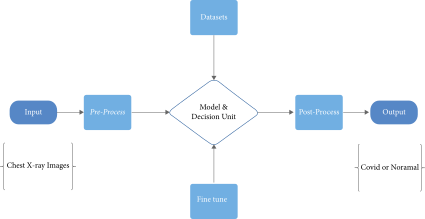
\includegraphics{assets/block.png}
    \caption{Block Diagram~\cite{Uddin2021} of the Proposed System}
\end{figure}

\subsection{Data Collection/Input:}

The data set is collected from different sources. We have proposed a framework that can effectively detect COVID-19 cases by evaluating the chest x-ray images. The image data are collected from different websites such as Radiopedia.org and Figure1.com. The random images are studied and divided into Normal image and Covid image. This data set is further converted into training and testing with the split of 70\% data for training of proposed deep learning model and 30\% data for testing purpose. 

\subsection{Data pre-processing }

Due to inconsistency of the dataset, the X-ray images are of different sizes. So, the all the images are converted to the same size. Also, splitting dataset process and data augmentation technique comes under data pre-processing. Final input to the proposed model is prepared. 

\section{Expected Outcomes}

The research study will explore different architectures for generating a valid classifier using CXR images. The research will produce a valid model which will be trained and tested for CXR images obtained from different labs. It shall classify the image report for the presence of \acrfull{cov} damages(pertaining damage). It will be further developed to predict the critical damage stage where a patient may need to be hospitalized.
\section{Timeline of the Study}


\begin{center}
    
    \begin{ganttchart}[
            hgrid, 
            vgrid,
            x unit=1cm,
        ]{0}{10}
        \gantttitle{2022}{11} \\
        \gantttitlelist{0,...,10}{1} \\
        \ganttgroup{Idea Incubation}{0}{1} \\
        \ganttbar{Generate Project Ideas}{0}{1} \\
        \ganttbar{Literature Review and Case Study}{0}{1} \\
        \ganttbar{Make Research Proposal}{1}{1} \\
        \ganttgroup{Research}{1}{7} \ganttnewline
        \ganttbar{Research Granted}{1}{1.5} \ganttnewline
        \ganttmilestone{Data Collection: Nepal CXR Images}{2} \ganttnewline
        \ganttlinkedbar{Deep Learning Model Development}{3}{4} \ganttnewline
        \ganttbar{Training and Testing}{2}{4} \ganttnewline
        \ganttbar{Experiment}{3}{5} \ganttnewline
        \ganttbar{Result Analysis and Validation}{5}{6} \ganttnewline
        \ganttbar{Documentation}{6}{7} \ganttnewline
        \ganttlink{elem5}{elem6}
    \end{ganttchart}
\end{center}

\section{Proposed Budget}

\begin{table}[!ht]
    \centering
    \begin{tabular}{|l|r|}
    \hline
        Total Budget & 100000 \\ \hline
        Data Collection (Digitization of CXR images) & 25000 \\ \hline
        Visits to specialists (Transportation and Misc.) & 10000 \\ \hline
        Cloud Computing Resource & 60000 \\ \hline
        Documentation & 5000 \\ \hline
    \end{tabular}
\end{table}
% \label{}

%% The Appendices part is started with the command \appendix;
%% appendix sections are then done as normal sections
%% \appendix

%% \section{}
%% \label{}

%% References
%%
%% Following citation commands can be used in the body text:
%% Usage of \cite is as follows:
%%   \cite{key}         ==>>  [#]
%%   \cite[chap. 2]{key} ==>> [#, chap. 2]
%%

%% References with BibTeX database:

\bibliographystyle{elsarticle-num}
\bibliography{pages/ref}

% \newpage
% \section{Annex}



%% Authors are advised to use a BibTeX database file for their reference list.
%% The provided style file elsarticle-num.bst formats references in the required Procedia style

%% For references without a BibTeX database:

% \begin{thebibliography}{00}

%% \bibitem must have the following form:
%%   \bibitem{key}...
%%

% \bibitem{}

% \end{thebibliography}

\end{document}

%%
%% End of file `ecrc-template.tex'. 